%cs4fIntro.tex


\section{Computer Science for Future}
\begin{frame}{}
\hspace*{\fill}

\includegraphics[width=.8\textwidth]{CS4Flogo.png}

\hspace*{\fill}
\end{frame}

\begin{frame}{\CSfF \ Computer Science for Future}
Initiativen  des Klimaschutzes und der Nachhaltigkeit  \\\hspace*{\fill}           (aus Sicht der Informatik)

\begin{itemize}
	\item in das Curriculum,
	\item mit unseren Kontakten aus Industrie und Gesellschaft,
	\item in die Forschung und
	\item die Organisation zu integrieren.
\end{itemize}
\vfill


Getragen von denen, die das wollen\\
Student*innen, Mitarbeiter*innen und Professor*innen\\ \vfill
Veränderungsprozess in unterschiedlicher Granularität \CSfF \ für
\begin{itemize}
	\item Repräsentation, Information und Koordinierung
	\item Maßnahmen umsetzen und unterstützen
	\item Verstetigung und Förderung vorantreiben
	\end{itemize}
\end{frame}

\begin{frame}{Mehr Infos??!!}
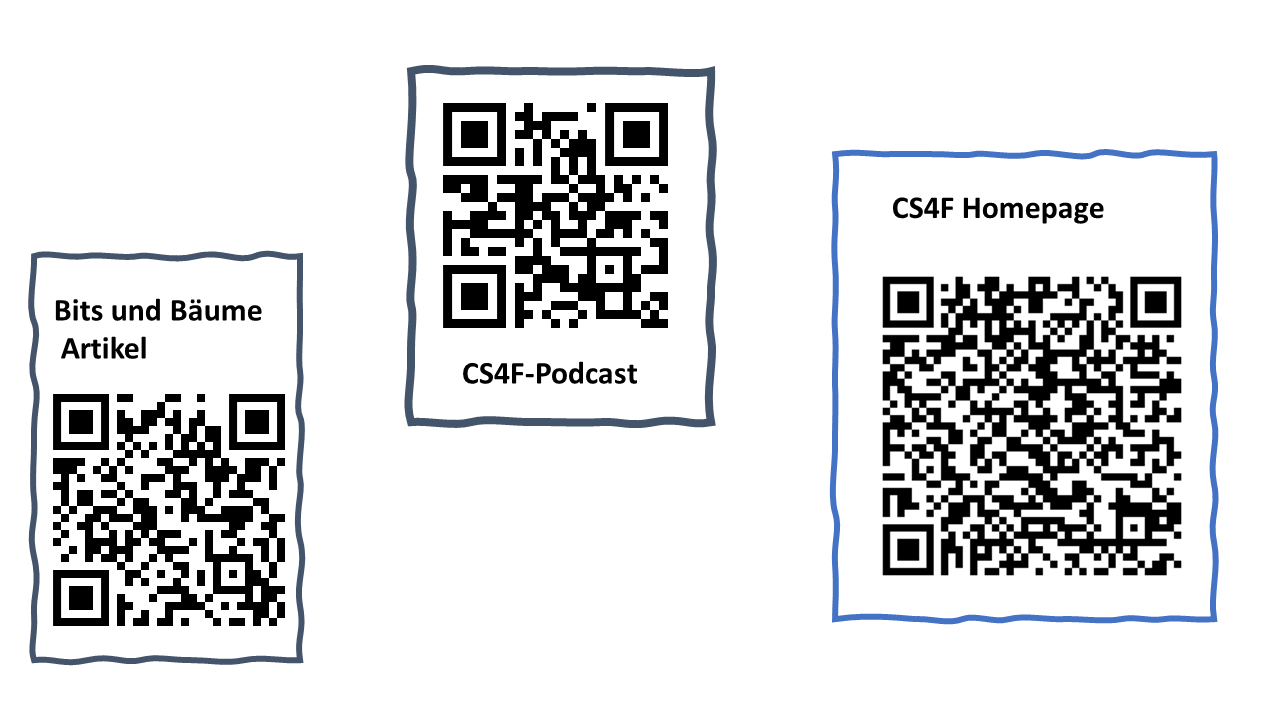
\includegraphics[width=.9\textwidth]{alle_QR_CS4F.png}

\end{frame}
